\documentclass[12pt]{article}

\usepackage{sbc-template}
\usepackage{graphicx,url}
\usepackage[utf8]{inputenc}
\usepackage[brazil]{babel}
\usepackage{lipsum}
%\usepackage[latin1]{inputenc}  
\usepackage{amsmath}
\usepackage[portuguese,ruled,vlined]{algorithm2e}
%\usepackage[portuguese,ruled,vlined,linesnumbered]{algorithm2e}
\usepackage{blindtext}
\usepackage{xcolor}
\usepackage{caption}
\usepackage{subcaption}
\usepackage{colortbl}
\usepackage{adjustbox}
\usepackage{tikz}
\usepackage{pgf}
\usepackage{multirow}
\usepackage{pgfplots}
\usepackage{amsmath}
     
\sloppy

\title{Componentes Conexos em Processador Multicore}
\author{Patreze A. Chita \inst{1}, Nahri. B. Moreano\inst{1}}
\address{Faculdade de Computação -- Universidade Federal do Mato Grosso do Sul (UFMS) \\ Caixa Postal 549 -- 79.070.900 -- Campo Grande -- MS -- Brazil
\email{patrezechita@gmail.com, nahri@facom.ufms.br}
}

\begin{document} 

\maketitle

%\begin{abstract}
%  This meta-paper describes the style to be used in articles and short papers
%  for SBC conferences. For papers in English, you should add just an abstract
%  while for the papers in Portuguese, we also ask for an abstract in
%  Portuguese (``resumo''). In both cases, abstracts should not have more than
%  10 lines and must be in the first page of the paper.
%\end{abstract}
     
\begin{resumo} 
Lorem ipsum dolor sit amet, consectetur adipiscing elit. Ut bibendum consectetur facilisis. Duis ut elit sed elit commodo pellentesque. Aenean pellentesque diam et lectus congue, porta ultricies enim varius. Praesent turpis velit, aliquam non venenatis ut, posuere egestas tellus. Etiam vel risus et ante pulvinar vulputate. Ut nec enim eu quam scelerisque tincidunt.
\end{resumo}

\section{Introdução}
{\color{gray}\lipsum[1]}

\section{Algoritmos Sequencial e Paralelo para Componentes Conexos}


\subsection{Algoritmo Sequencial Baseado em Busca em Profundidade}

Inicialmente, uma maneira natural de se resolver o problema dos componentes conexos é executando uma busca em profundidade em um determinado grafo. O resultado disso é uma floresta composta por várias árvores, que são por definição conexas (existe pelo menos um caminho entre dois vértices quaisquer da árvore) e acíclicas. Portanto, um algoritmo de busca em profundidade levemente modificado pode resolver sequencialmente o problema dos componentes conexos. Essa afirmação é corroborada por Grama e Sedgewick (citar). O autor do livro Introduction to Parallel Computing apresenta duas maneiras de se resolver o problema, utilizando busca em profundidade (sequencial) e esboça uma ideia de como seria um algoritmo paralelo, dividindo a busca em profundidade entre os processadores e depois unindo os conjuntos gerados.

Como resultado de uma busca em profundidade, todo vértice que pertence a uma mesma árvore da solução da busca, está em um mesmo componente do grafo. Facilmente nota-se essa afirmação pois partindo de um vértice, será acessado outro que compartilha uma aresta, logo existe um caminho entre esses dois vértices. A modificação necessária no algoritmo de busca em profundidade é que, toda vez que um vértice é visto pela busca, todos os próximos vértices (acessados a partir deste) estarão no mesmo componente do grafo. O algoritmo \ref{alg_seq} ilustra o funcionamento sequencial implementado (conhecido na literatura) da busca em profundidade com a modificação para se armazenar a informação de qual componente pertence cada vértice.

\begin{algorithm}[htp!]
    \DontPrintSemicolon
    \SetArgSty{textnormal}
    \caption{Algoritmo sequencial para componentes conexos}
    \label{alg_seq}
    \SetKwProg{ComponentesConexos}{ComponentesConexos}{}{}
    \ComponentesConexos{{\normalfont(grafo G = (V, E))}}
	{
        nComponentes $\gets$ 0\;
        \ParaCada{vértice v $\in$ V}
        {
            visitado[v] $\gets$ FALSO\;
        }
        \ParaCada{vértice v $\in$ V}
        {
            \Se{visitado[v] = FALSO}
            {
                \textbf{DFS}(v)\;
                nComponentes $\gets$ nComponentes + 1\;
            }
        }
    }
    \SetKwProg{DFS}{DFS}{}{}
    \DFS{{\normalfont(vértice v)}}
    {
        componente[v] $\gets$ nComponentes\; 
        visitado[v] $\gets$ VERDADEIRO\;
        \ParaCada{vértice u $\in$ Adj[v]}
        {
            \Se{visitado[u] = FALSO}
            {
                \textbf{DFS}(u)\;
            }
        }
    }
\end{algorithm}

\subsection{Algoritmo Paralelo Baseado em Busca em Profundidade e nas Operações Union/Find}

Em~\cite{Grama:2003} uma ideia de como paralelizar esse processo sequencial da busca em profundidade é apresentada. Sua sugestão, mesmo sendo bem alto nível, é suficiente para entender o funcionamento do algoritmo paralelo. Primeiramente, deve-se dividir a matriz de adjacências do grafo por todos os processadores, assim sendo, cada processador vai receber um ``pedaço'' do grafo no qual irá realizar uma busca em profundidade. Após esse procedimento, todos conjuntos gerados pela busca serão unidos par a par, até sobrar somente um conjunto. O resultado será semelhante ao de executar a busca em profundidade de maneira sequencial. O algoritmo 2 ilustra os passos desse algoritmo paralelo do grama.

\begin{algorithm}[htp!]
    \DontPrintSemicolon
    \SetArgSty{textnormal}
    \newcommand\mycommfont[1]{\small\ttfamily{#1}}
	\SetCommentSty{mycommfont}
    \caption{Algoritmo paralelo para componentes conexos}
    \label{alg_grama}
    \SetKwFor{ForPar}{para cada}{fa\c{c}a em paralelo}{fim para cada}
    \SetKwProg{ComponentesConexosPar}{ComponentesConexosParalelo}{}{}
    \ComponentesConexosPar{{\normalfont(grafo G = (V, E))}}
    {
        p $\gets$ número de processadores\;
        %Divide vértices de $V$ em $p$ partes de $\sim|V|/p$ vértices\;
        divida a matriz de adjacência de G em p faixas\;
        atribua cada faixa da divisão a um dos p processadores\;
        %\tcp{Executar DFS em paralelo, gerando p florestas}
        \ForPar{processador $\text{p}_\text{i}$}
        {
            $\text{E}_\text{i} \gets$ arestas da faixa da matriz de adjacência atribuída a $\text{p}_\text{i}$\;
            %$\text{G}_\text{i} \gets$ subgrafo de G induzido por $\text{E}_\text{i}$\;
            defina subgrafo $\text{G}_\text{i}$ = (V, $\text{E}_\text{i}$)\;
            execute \textbf{DFS}($\text{G}_\text{i}$) produzindo floresta $\text{F}_\text{i}$\;
        }

        una florestas $\text{F}_\text{i}$, par a par, até restar uma única floresta F\;
        
        %\tcp{Para cada árvore $A$ $\in$ $F$, vértices de $A$ estão no mesmo componente}
        %\tcp{todos os vértices de uma mesma árvore de F pertencem ao mesmo componente}
    }
\end{algorithm}

\section{Solução Paralela para Componentes Conexos para Processador Multicore}

Tendo em mãos a sugestão do algoritmo paralelo~\cite{Grama:2003}, implementamos uma versão nossa do algoritmo dado as especificidades da linguagem e da experiencia do autor deste trabalho. Primeiramente, utilizamos listas de adjacências para representar os grafos e não matriz de adjacência como sugere o autor. A linguagem utilizada é C e para paralelizar o código, foi utilizado o OpenMP~\cite{OpenMP:2018}. Como entrada, o algoritmo implementado recebe um arquivo contendo todas as arestas do grafo de entrada, ao ler esse conjunto de arestas, o algoritmo monta a lista de adjacências que será utilizada pela busca em profundidade.
 
Com a lista de adjacências pronta, é feito um cálculo para dividir o mais igual possível a quantidade de vértices para cada processador, na intenção de dividir igualmente a carga de trabalho. Sendo assim, cada processador irá possuir um subgrafo que será gerado pelos vértices da lista de adjacência designados ao processador.
 
A busca em profundidade é executada, cada processador, ao ver um vértice irá marcar esse vértice em um componente e todos os outros vértices que podem ser vistos a partir deste, estarão no mesmo componente. É utilizado uma estrutura de dados chamada componente, onde cada processador possui o índice do componente ao qual pertence. Também durante a busca em profundidade, é necessário que seja armazenado a aresta da qual o processador ``viu''. Utilizamos a estrutura floresta para que seja guardado os pares de arestas vistos durante a busca. O resultado da busca em profundidade que cada processador executa paralelamente é a floresta e o índice do componente de cada vértice, mas veja que, um processador guarda um índice de um componente de um vértice que ele não viu (por padrão, o índice do próprio vértice), iremos resolver essa inconsistência no próximo passo.
 
Feita a busca em profundidade, é hora de unir todos os dados dos processadores. Como essa união é feita entre dois processadores (par a par), utilizamos a definição de processador da esquerda e processador da direita para se referir ao par de processadores. A união das florestas é simples e ocorre da seguinte maneira: para cada aresta do processador da direita, o processador da direita faz um find nos componentes destes dois vértices que compõem a aresta. Caso o find resulte em componentes diferentes, significa que para o processador da direita estes dois vértices estão em um mesmo componente no grafo (pois ele viu isso na busca em profundidade) mas o processador da esquerda não viu esses dois vértices na sua busca em profundidade e então ele deve atualizar o índice dos dois vértices e na sua estrutura floresta, adicionar a aresta, sendo esse processo o union. Caso o processador da esquerda, ao fazer o find, retorne que os dois vértices estão no mesmo componente, então simplesmente ignora a aresta do processador da direita.
 
Esse procedimento é repetido para todas as arestas que o processador da direita possui em sua estrutura floresta. Após concluído esse procedimento, teremos em todos os processadores da esquerda, os valores atualizados e nos da direita, os valores que não serão mais uteis, portanto, metade dos processadores não serão mais utilizados para o próximo passo, que é executar novamente a união dos conjuntos com os processadores que ainda restaram, par a par. Ao final desse processo, teremos apenas dois processadores e o processador da esquerda deste ultimo procedimento terá a informação completa sobre os componentes conexos do grafo de entrada. A Figura~\ref{1} ilustra a execução deste algoritmo, o qual é representado nos Algoritmos~\ref{3} e \ref{4}.

\begin{figure}[htp!]
	\centering
	\subcaptionbox{}[.32\textwidth]
	{
		\resizebox{0.3\textwidth}{!}
        {
			\begin{tikzpicture}
			[scale=1,auto=left,every node/.style={circle,fill=gray!20}]
				\node (v0) at (0,4) {0};
				\node (v6) at (0,0) {6};
				\node (v3) at (0,2) {3};
				\node (v2) at (2,4) {2};
				\node (v1) at (6,4) {1};
				\node (v4) at (6,2) {4};
				\node (v5) at (4,2) {5};
				\node (v7) at (6,0) {7};
				\node (v8) at (2,0) {8};
				\node (v9) at (4,0) {9};
				\node [fill=white!0](x) at (0,-1) {}; %vértice invisível para alinhar 
				\foreach \from/\to in {v0/v3,v3/v6,v3/v2,v0/v2,v1/v4,v4/v5,v4/v7,v8/v9}
				\draw[line width=1.5pt] (\from) -- (\to);
			\end{tikzpicture}
		}
	}
	\subcaptionbox{}[.32\textwidth]
	{
		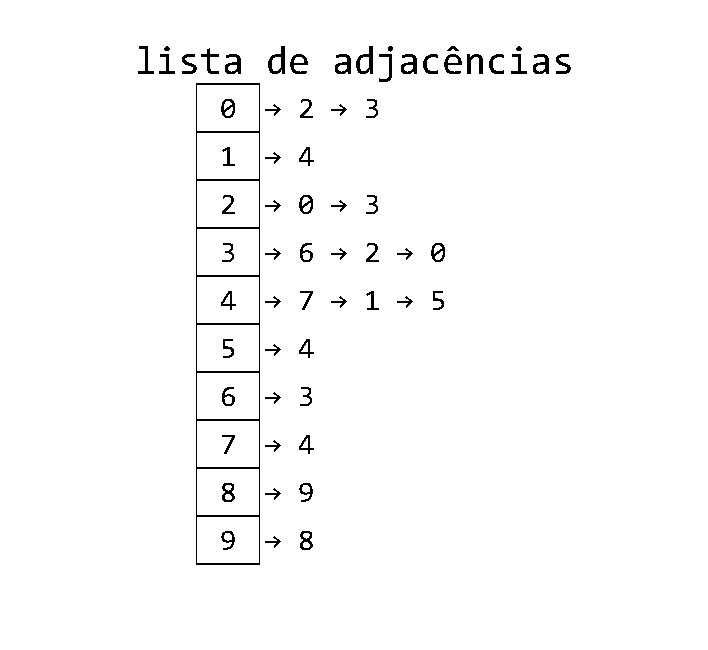
\includegraphics[width=\linewidth]{figB.pdf}
	}
	\subcaptionbox{}[.32\textwidth]
	{
		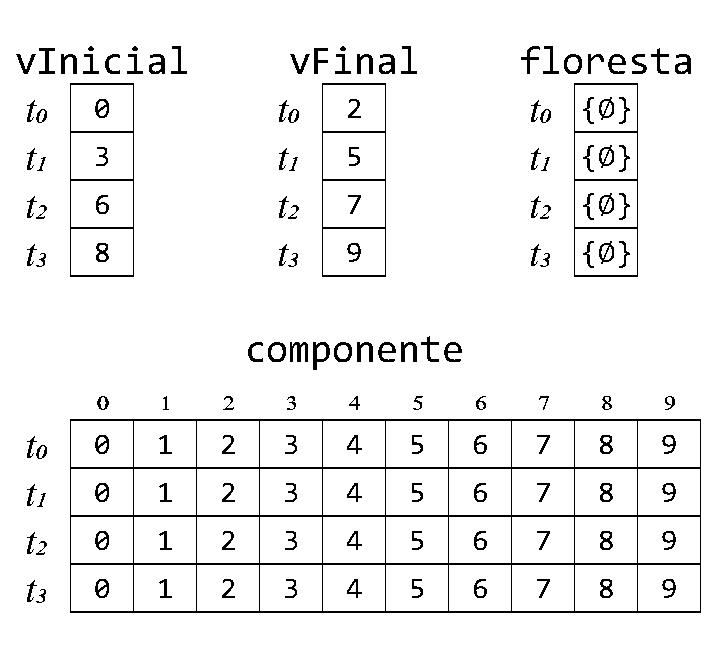
\includegraphics[width=\linewidth]{figC.pdf}
	}
	\subcaptionbox{}[.32\textwidth]
	{
		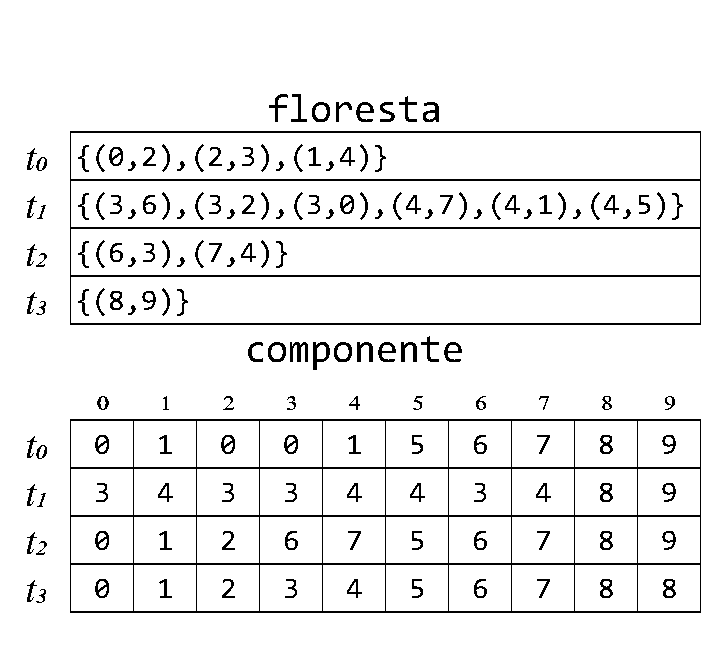
\includegraphics[width=\linewidth]{figD.pdf}
	}
	\subcaptionbox{}[.32\textwidth]
	{
		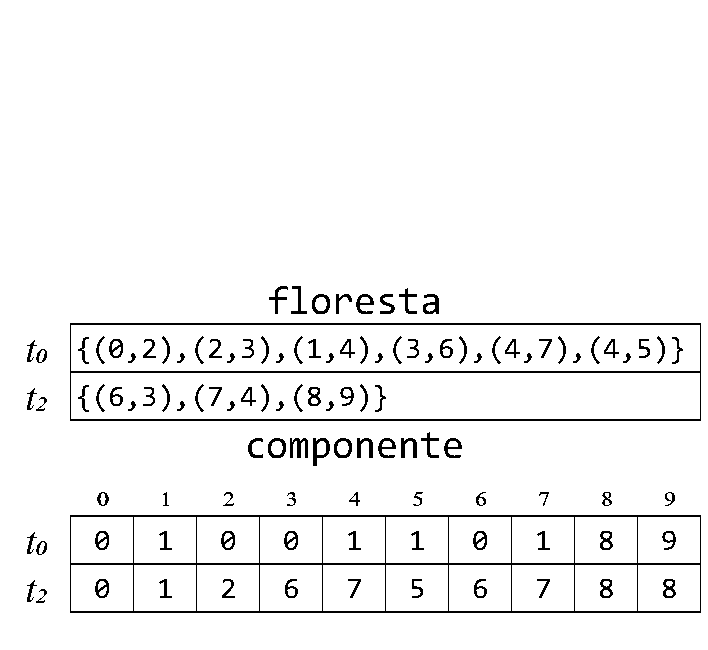
\includegraphics[width=\linewidth]{figE.pdf}
	}
	\subcaptionbox{}[.32\textwidth]
	{
		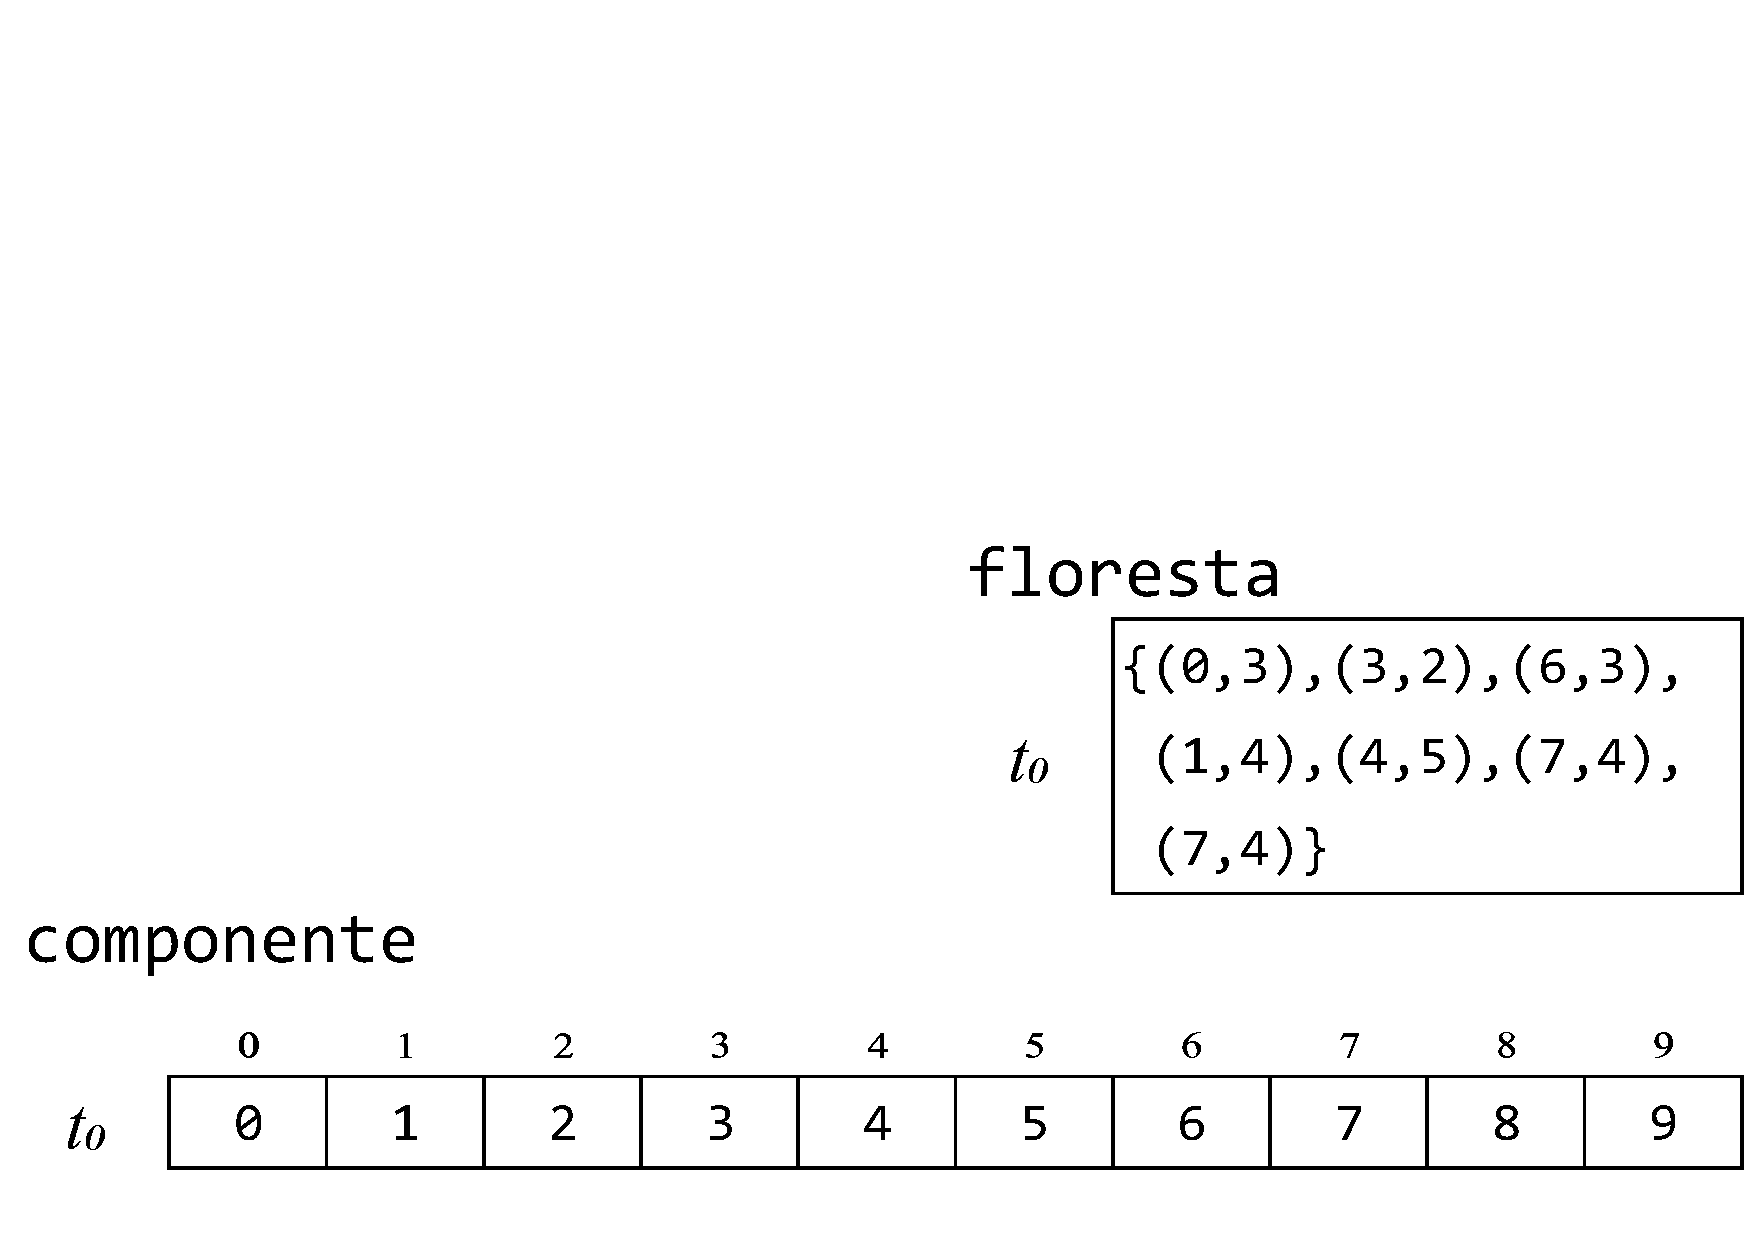
\includegraphics[width=\linewidth]{figF.pdf}
	}
	\caption{Execução da implementação do algoritmo paralelo. (a) Representação gráfica de G=(V, E). (b) A lista de adjacências do grafo G. (c) Estado das estruturas antes de iniciar o DFS paralelo. (d) Estado das estruturas após terminar de executar o DFS em paralelo. (e) Estado das estruturas após fazer a primeira rodada de uniões em paralelo. (f) Estado das estruturas após fazer a segunda rodada de uniões, sendo que a \emph{thread} 0 possui o resultado do algoritmo.}
\end{figure}

\begin{algorithm}[htp!]
    \DontPrintSemicolon
    \SetArgSty{textnormal}
    \newcommand\mycommfont[1]{\small\ttfamily{#1}}
	\SetCommentSty{mycommfont}
    %\SetAlCapNameFnt{\small} %tamanho nome do algoritmo
    \caption{Implementação do algoritmo paralelo para componentes conexos}
    \label{alg_par1}
    \SetKwProg{ComponentesConexosPar}{ComponentesConexosParalelo}{}{}
    \SetKwFor{ForPar}{para}{fa\c{c}a em paralelo}{fim para cada}
    \ComponentesConexosPar{{\normalfont(grafo G = (V, E))}}
    {
    	\tcp{Divida os vértices pelas threads}
        nTh $\gets$ número de threads\;
        nVerticesExtra $\gets |\text{V}|$ -- ($\lfloor \frac{|\text{V}|}{\text{nTh}} \rfloor$ $\times$ nTh)\;
        \ForPar{$t \gets 0$ \Ate $nTh-1$}
        {
            \eSe{t $<$ nVerticesExtra}
            {
                vInicial[t] $\gets$ t $\times$ $\lceil\frac{|\text{V}|}{\text{nTh}}\rceil$\;
                vFinal[t] $\gets$ vInicial[t] + $\lceil\frac{|\text{V}|}{\text{nTh}}\rceil$ -- 1\;
            }
           {
                vInicial[t] $\gets$ t $\times$ $\lfloor\frac{|\text{V}|}{\text{nTh}}\rfloor$ + nVerticesExtra\;
                vFinal[t] $\gets$ vIncial[t] + $\lfloor\frac{|\text{V}|}{\text{nTh}}\rfloor$ -- 1\;
            }
        }
        \tcp{Execute DFS em paralelo, gerando nTh florestas}
        \ParaCada{vértice v $\in$ V}
        {
            visitado[v] $\gets$ FALSO\;
        }
        \ForPar{t $\gets$ 0 \Ate nTh -- 1}
        {
            \ParaCada{vértice v $\in$ V}
            {
                componente[t][v] $\gets$ v\;
            }
            floresta[t] $\gets$ \{$\emptyset$\}\;
            \Para{v $\gets$ vInicial[t] \Ate vFinal[t]}
            {
                \Se{visitado[v] = FALSO}
                {
                    raiz $\gets$ v\;
                    \textbf{DFS}(t, v, raiz)\;
                }
            }
        }
        \tcp{Una pares de florestas em paralelo}
        nPares $\gets \frac{\text{nTh}}{\text{2}}$\;
        \Para{i $\gets$ 0 \Ate $\log_2\!\text{(nTh)}$ -- 1}
        {
            \ForPar{t $\gets$ 0 \Ate nPares -- 1}
            {
                thEsquerda $\gets$ t $\times$ $\text{2}^{\text{i+1}}$\;
                thDireita $\gets$ thEsquerda + $\text{2}^\text{i}$\;
                
                \ParaCada{aresta (v, u) $\in$ floresta[thDireita]}
                {
                    \textbf{Union}(thEsquerda, v, u)\;
                }
            }
            nPares $\gets \frac{\text{nPares}}{\text{2}}$\;
        }
    }
    \SetKwProg{DFS}{DFS}{}{}
    \DFS{{\normalfont(thread t, vértice v, vértice raiz)}}
    {
        componente[t][v] $\gets$ raiz\;
        
        \ParaCada{vértice u $\in$ Adj[v]}
        {
            floresta[t] $\gets$ floresta[t] $\cup$ \{(v, u)\}\;
            componente[t][u] $\gets$ raiz\;
            
            \Se{vInicial[t] $\le$ u \textbf{\upshape e} u $\le$ vFinal[t]}
            {
                \Se{visitado[u] = FALSO}
                {
                    \textbf{DFS}(t, u, raiz)\;
                }
            }
        }
        visitado[v] $\gets$ VERDADEIRO\;
    }
\end{algorithm}
    
\begin{algorithm}[h]
    \DontPrintSemicolon
    \SetArgSty{textnormal}
    \caption{Operações Union e Find}
    \label{alg_par2}
    \SetKw{Return}{retorna}
    \SetKwProg{UNION}{Union}{}{}
    \UNION{{\normalfont(thread t, vértice v, vértice u)}}
    {
        vComponente $\gets$ \textbf{Find}(t, v)\;
        uComponente $\gets$ \textbf{Find}(t, u)\;
        min $\gets$ \textbf{Mínimo}(vComponente, uComponente)\;
		max $\gets$ \textbf{Máximo}(vComponente, uComponente)\;
        \Se{vComponente $\neq$ uComponente}
        {
            \ParaCada{vértice i $\in$ V}
            {
                \Se{componente[t][i] = max}
                {
                    componente[t][i] $\gets$ min\;
                }
            }
            floresta[t] $\gets$ floresta[t] $\cup$ \{(v, u)\}\;
        }
    }
    \SetKwProg{FIND}{Find}{}{}
    \FIND{{\normalfont(thread t, vértice v)}}
    {
        \Return componente[t][v]\;
    }
\end{algorithm}

\section{Resultados e Análise}

Para mensurar o desempenho dos dois algoritmos implementados, utilizamos um grafo de entrada aleatório com vários tamanhos, sendo eles 5.000, 10.000, 15.000 e 25.000 vértices. Apesar de o tamanho ser aparentemente pequeno, a busca em profundidade analisa todas as arestas do grafo e não somente os vértices, logo, para um grafo k-completo de 25.000 vértices teremos 312.487.500 arestas. Como os grafos são aleatórios, dividimos os mesmos em densidades (quantidade de arestas do grafo em relação a quantidade máxima de arestas possíveis), sendo elas 10\%, 25\%, 50\%, 75\% e 100\%. Um grafo de 5.000 vértices e densidade de 25\% tem 3.124.375 arestas já que, caso fosse definido uma densidade de 100\%, este mesmo grafo possuiria 12.497.500 arestas.
A execução do algoritmo se deu em uma máquina DELL PRECISION (Intel Xeon CPU E5-1620 v3 3.5GHz, 4 núcleos, 8 threads, 32GB de RAM) alocada na FACOM. Os gráficos abaixo ilustram os testes de desempenho.

\begin{figure}[htp!]
    \centering
    \begin{minipage}{.48\textwidth}
        \centering
        \resizebox{\textwidth}{!}
        {
			\begin{tikzpicture}
			\begin{axis}[
				%title={Execução alg par 25k com várias threads},
				legend pos=north west,
				xlabel={quantidade de vértices},
				%legend style={at={(0.5,-0.20)},anchor=north,legend columns=-1},
				%symbolic x coords={a,b,c,d},
				ylabel={tempo de execução (s)},
				xtick=data,
				symbolic x coords={5K, 10K, 15K, 25K}]
				\addplot coordinates {
					(5K,2.8425)(10K,12.9809)(15K,35.0820)(25K,105.7478)};
				\addplot coordinates {
					(5K,0.9850)(10K,4.2318)(15K,10.5094)(25K,30.9745)};
			\legend{Sequencial, Paralelo}
			\end{axis}
			\end{tikzpicture}
		}
        \caption{Tempo de execução, densidade fixada em 100\% e paralelo com 16 \emph{threads}}
    \end{minipage}\hfill%
    \begin{minipage}{.48\textwidth}
        \centering
        \resizebox{\textwidth}{!}
        {
			\begin{tikzpicture}
			\begin{axis}[
				%title={Execução alg par 25k com várias threads},
				legend pos=north west,
				xlabel={densidade do grafo},
				%legend style={at={(0.5,-0.20)},anchor=north,legend columns=-1},
				%symbolic x coords={a,b,c,d},
				ylabel={tempo de execução (s)},
				xtick=data,
				symbolic x coords={5\%, 25\%, 50\%, 75\%, 100\%}]
				\addplot coordinates {
					(5\%,3.7357)(25\%,22.9317)(50\%,50.8209)(75\%,77.6357)(100\%,105.7478)};
				\addplot coordinates {
					(5\%,1.3433)(25\%,8.1235)(50\%,16.6858)(75\%,24.3761)(100\%,30.9745)};
			\legend{Sequencial, Paralelo}
			\end{axis}
			\end{tikzpicture}
		}
        \caption{Tempo de execução, tamanho fixado em 25K e paralelo com 16 \emph{threads}}
    \end{minipage}
\end{figure}

Na figura 2 é analisado o tempo de execução dos dois algoritmos (sequencial e paralelo) em relação ao tamanho de vértices da entrada (sendo o grafo de entrada k-completo, ou seja, com densidade de 100\%). Já na figura 3, temos um grafo de entrada de tamanho fixo (25.000 vértices) variando sua densidade.

\begin{figure}[htp!]
    \centering
    \begin{minipage}{.48\textwidth}
        \centering
        \resizebox{\textwidth}{!}
        {
			\begin{tikzpicture}
			\begin{axis}[
				%title={Execução alg par 25k com várias threads},
				legend style={at={(0.5,1.15)},anchor=north,legend columns=-1},
				xlabel={quantidade de vértices},
				%legend style={at={(0.5,-0.20)},anchor=north,legend columns=-1},
				%symbolic x coords={a,b,c,d},
				ylabel={\emph{speedup}},
				xtick=data,
				symbolic x coords={5K, 10K, 15K, 25K}]
				\addplot coordinates {
					(5K,2.0066)(10K,2.5546)(15K,2.5800)(25K,2.7810)};
				\addplot coordinates {
					(5K,2.7384)(10K,2.7336)(15K,2.6243)(25K,2.8229)};
				\addplot coordinates {
					(5K,2.6475)(10K,2.7354)(15K,2.7931)(25K,3.0458)};
				\addplot coordinates {
					(5K,2.7349)(10K,2.8928)(15K,3.0592)(25K,3.1849)};
				\addplot coordinates {
					(5K,2.8858)(10K,3.0675)(15K,3.3382)(25K,3.4140)};
			\legend{5\%, 25\%, 50\%, 75\%, 100\%}
			\end{axis}
			\end{tikzpicture}
		}
        \caption{\emph{Speedup} paralelo em relação ao sequencial, paralelo com 16 \emph{threads}}
    \end{minipage}\hfill%
    \begin{minipage}{.48\textwidth}
        \centering
        \resizebox{\textwidth}{!}
        {
			\begin{tikzpicture}
			\begin{axis}[
				legend pos=north west,
				%legend style={at={(0.5,1.15)},anchor=north,legend columns=-1},
				%xlabel={densidade do grafo},
				%legend style={at={(0.5,-0.20)},anchor=north,legend columns=-1},
				%symbolic x coords={a,b,c,d},
				ylabel={\emph{speedup}},
				xlabel={densidade do grafo},
				xtick=data,
				symbolic x coords={5\%, 25\%, 50\%, 75\%, 100\%}]
				\addplot coordinates {
					(5\%,2.0066)(25\%,2.7384)(50\%,2.6475)(75\%,2.7349)(100\%,2.8858)};
				\addplot coordinates {
					(5\%,2.5546)(25\%,2.7336)(50\%,2.7354)(75\%,2.8928)(100\%,3.0675)};
				\addplot coordinates {
					(5\%,2.5800)(25\%,2.6243)(50\%,2.7931)(75\%,3.0592)(100\%,3.3382)};
				\addplot coordinates {
					(5\%,2.7810)(25\%,2.8229)(50\%,3.0458)(75\%,3.1849)(100\%,3.4140)};
			\legend{5K, 10K, 15K, 25K}
			\end{axis}
			\end{tikzpicture}
		}
        \caption{\emph{Speedup} paralelo em relação ao sequencial, paralelo com 16 \emph{threads}}
    \end{minipage}
\end{figure}

A figura 4 e 5 temos os speedups do algoritmo paralelo em relação ao sequencial. Nota-se aqui mais facilmente como há também um ganho de performance em relação ao grafo de menor tamanho (visto que é mais difícil enxergar essa diferença na figura 2 e 3).

\begin{figure}[h]
    \centering
    \begin{minipage}{.48\textwidth}
        \centering
        \resizebox{\textwidth}{!}
        {
			\begin{tikzpicture}
			\begin{axis}[
				legend pos=north west,
				xlabel={quantidade de vértices},
				%legend style={at={(0.5,-0.20)},anchor=north,legend columns=-1},
				%symbolic x coords={a,b,c,d},
				ylabel={tempo de execução (s)},
				xtick=data,
				symbolic x coords={5K, 10K, 15K, 25K}]
				\addplot coordinates {
					(5K,2.0038)(10K,8.4621)(15K,21.8479)(25K,64.3706)};
				\addplot coordinates {
					(5K,1.2820)(10K,5.8591)(15K,14.8007)(25K,41.4975)};
				\addplot coordinates {
					(5K,1.0018)(10K,4.3181)(15K,10.5758)(25K,31.0767)};
				\addplot coordinates {
					(5K,0.9850)(10K,4.2318)(15K,10.5094)(25K,30.9745)};
			\legend{2 $th$,4 $th$,8 $th$, 16 $th$}
			\end{axis}
			\end{tikzpicture}
		}
        \caption{Tempo de execução, densidade fixada em 100\%}
    \end{minipage}\hfill%
    \begin{minipage}{.48\textwidth}
        \centering
        \resizebox{\textwidth}{!}
        {
			\begin{tikzpicture}
			\begin{axis}[
				legend pos=north west,
				xlabel={densidade do grafo},
				%legend style={at={(0.5,-0.20)},anchor=north,legend columns=-1},
				%symbolic x coords={a,b,c,d},
				ylabel={tempo de execução (s)},
				%xtick=data,
				symbolic x coords={5\%, 25\%, 50\%, 75\%, 100\%}]
				\addplot coordinates {
					(5\%,2.4396)(25\%,15.6663)(50\%,33.4889)(75\%,51.2299)(100\%,64.3706)
				};
				\addplot coordinates {
					(5\%,1.6939)(25\%,11.2393)(50\%,22.2700)(75\%,35.0567)(100\%,41.4975)
				};
				\addplot coordinates {
					(5\%,1.3561)(25\%,8.1547)(50\%,16.7268)(75\%,24.5019)(100\%,31.0767)
				};
				\addplot coordinates {
					(5\%,1.3433)(25\%,8.1235)(50\%,16.6858)(75\%,24.3761)(100\%,30.9745)
				};
			\legend{2 $th$,4 $th$,8 $th$, 16 $th$}
			\end{axis}
			\end{tikzpicture}
		}
        \caption{Tempo de execução, tamanho fixado em 25K}
    \end{minipage}
\end{figure}

A fim de medir diferentes desempenhos em relação a quantidade de threads, a figura 6 e 7 ilustram o tempo de execução do algoritmo utilizando diferentes quantidades de threads. Essa medição é interessante para ilustrar o desempenho do algoritmo em relação ao seu potencial de paralelismo. 





\section{Conclusão}

{\color{gray}\lipsum[1]}

\cite{Sedgewick:2011} s \cite{Cormen:2009} and \cite{Grama:2003}


\bibliographystyle{sbc}
\bibliography{sbc-template}

\end{document}
